\section{NỘI DUNG VÀ PHƯƠNG PHÁP}

\subsection{Giới thiệu về benchmark NIKA}

NIKA được giới thiệu như một network arena để đánh giá AI Agent trong bài toán xử lý sự cố mạng~\citep{nika_arena2025}. Benchmark này giải quyết một khoảng trống quan trọng: trước đây việc đánh giá agent chẩn đoán mạng thường thiếu môi trường chuẩn hóa, khó tái lập và tốn nhiều công sức vận hành. Như minh họa trong Hình~\ref{fig:nika_overview}, NIKA cung cấp các kịch bản mạng có thể replay, giao diện agent--network rõ ràng và tập incident được thiết kế để kiểm tra khả năng phát hiện lỗi, định vị thiết bị lỗi và xác định nguyên nhân gốc rễ. Vì vậy, NIKA phù hợp với mục tiêu của đề tài: xây dựng một agent không chỉ trả lời bằng ngôn ngữ tự nhiên, mà còn phải sử dụng công cụ, thu thập bằng chứng và cải thiện qua nhiều lần xử lý sự cố.

\begin{center}
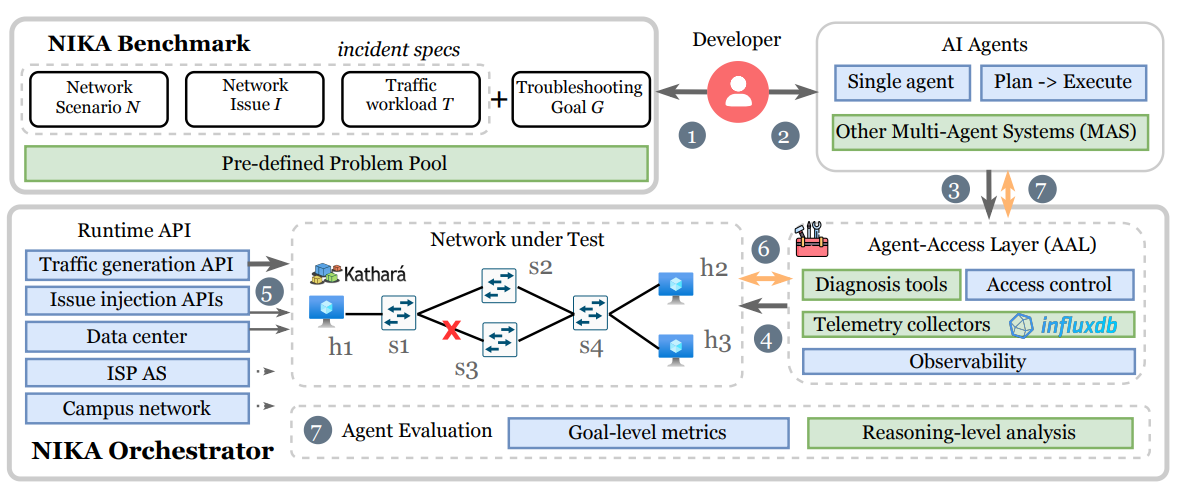
\includegraphics[width=\columnwidth]{figs/nika.png}
\captionof{figure}{Tổng quan benchmark NIKA cho đánh giá AI Agent trong xử lý sự cố mạng.}
\label{fig:nika_overview}
\end{center}

\subsection{Khung tổng quan hệ thống}

Hệ thống được xây dựng quanh một agent chẩn đoán có khả năng tương tác với môi trường mạng thông qua các công cụ MCP. Ở mức tổng quan, môi trường mạng cung cấp topology, thiết bị và dữ liệu quan sát; agent sử dụng các công cụ để kiểm tra trạng thái mạng; bộ chấm điểm đánh giá kết quả cuối cùng; và hai mô-đun tự tiến hóa cập nhật tri thức chẩn đoán sau mỗi episode. Hai mô-đun này gồm Procedural Memory để lưu kinh nghiệm dưới dạng quy trình chẩn đoán và Tool Refinement để cải thiện tài liệu công cụ dựa trên trace thực thi.

\subsubsection{Công cụ và công nghệ sử dụng}

Hệ thống sử dụng NIKA làm benchmark chính để tạo các incident mạng và chấm điểm kết quả chẩn đoán. Kathará~\citep{kathara2019} được dùng để ảo hóa topology bằng container, giúp khởi động lab, tiêm lỗi và tái lập môi trường một cách nhất quán. MCP/FastMCP~\citep{mcp2024} đóng vai trò lớp giao tiếp giữa agent và môi trường mạng: các thao tác như kiểm tra kết nối, đọc cấu hình, truy vấn telemetry hoặc nộp kết quả đều được chuẩn hóa thành công cụ. LangGraph/LangChain~\citep{langgraph2024} được dùng để điều phối workflow agent, trong đó các chiến lược chính gồm ReAct~\citep{react2023}, Plan \& Execute và Reflexion~\citep{reflexion2023}.

Ở tầng dữ liệu và mạng, hệ thống dùng InfluxDB để lưu telemetry, FRRouting~\citep{frr2021} cho các kịch bản định tuyến và P4/BMv2~\citep{p4lang2014} cho các kịch bản data-plane lập trình được. Phần triển khai được viết bằng Python 3.12 và quản lý môi trường bằng \code{uv}. Các nhóm công cụ MCP chính gồm Kathará Base, FRR, BMv2/P4, Telemetry, Task Management và Tool Evolution; mỗi nhóm tương ứng với một phần quan sát hoặc điều khiển cần thiết trong quá trình agent xử lý sự cố.

\subsubsection{Quy trình triển khai}

Quy trình triển khai bắt đầu từ việc chọn tập case trong benchmark, chuẩn bị cấu hình lab và xác định loại lỗi cần tiêm. Sau đó hệ thống khởi động môi trường, đưa agent vào vòng chẩn đoán và ghi lại toàn bộ trace gồm suy luận, lời gọi công cụ, quan sát trả về và kết luận cuối cùng. Các trace này vừa phục vụ chấm điểm, vừa là dữ liệu đầu vào cho hai mô-đun tự tiến hóa sau khi episode kết thúc.

Một episode chẩn đoán diễn ra theo trình tự: khởi động lab mạng, tiêm lỗi, chạy agent, thu thập trace gọi công cụ, nộp kết quả gồm \code{is\_anomaly}, \code{faulty\_devices}, \code{root\_cause\_name}, sau đó đánh giá và kích hoạt học ngoại tuyến. Với baseline, mỗi episode độc lập. Với evolved agent, bộ nhớ kỹ năng và tài liệu công cụ đã được tinh chỉnh từ các episode trước được nạp lại vào ngữ cảnh để hỗ trợ case tiếp theo.

Luồng xử lý được tách thành hai pha. Trong Diagnosis Phase, agent được quyền dùng đầy đủ công cụ để thu thập bằng chứng, kiểm tra giả thuyết và loại trừ nguyên nhân sai. Trong Submission Phase, agent chỉ còn công cụ nộp kết quả, nhờ đó giảm rủi ro vừa chẩn đoán vừa thay đổi kết luận cuối cùng một cách thiếu kiểm soát. Thiết kế này bám sát tinh thần ReAct, nơi suy luận và hành động công cụ được xen kẽ để giải quyết tác vụ nhiều bước, nhưng bổ sung lớp đánh giá sau episode để phục vụ học liên tục.

\subsection{Mô-đun Procedural Memory}

Procedural Memory được thiết kế để chuyển kinh nghiệm xử lý sự cố từ dạng lịch sử thụ động sang dạng quy trình có thể tái sử dụng~\citep{skillpro2024}. Trong các incident lặp lại hoặc có cấu trúc tương tự, agent không nên đọc lại toàn bộ trajectory cũ rồi suy luận lại từ đầu. Thay vào đó, hệ thống rút gọn kinh nghiệm thành các kỹ năng chẩn đoán có điều kiện kích hoạt rõ ràng, quy trình thực thi cụ thể và điều kiện dừng. Hình~\ref{fig:skillpro_overview} minh họa vòng đời này: trace sau episode được dùng để tạo hoặc cập nhật kỹ năng; ở episode tiếp theo, agent truy xuất kỹ năng phù hợp để định hướng chuỗi hành động công cụ.

\begin{center}
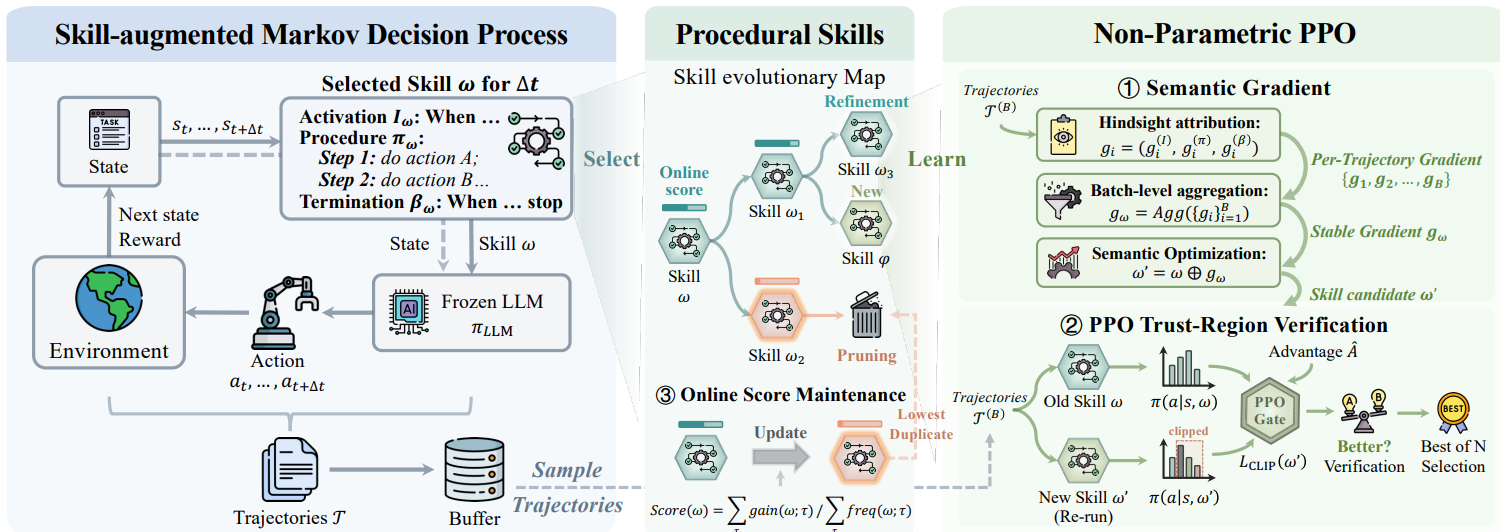
\includegraphics[width=\columnwidth]{figs/skillpro.png}
\captionof{figure}{Quy trình học kỹ năng tái sử dụng cho mô-đun Procedural Memory.}
\label{fig:skillpro_overview}
\end{center}

Mỗi kỹ năng được biểu diễn thành ba thành phần. \textit{Activation condition} mô tả tình huống nên gọi kỹ năng, chẳng hạn mất kết nối host, bất thường định tuyến BGP/OSPF hoặc lỗi liên quan đến switch P4/BMv2. \textit{Execution procedure} mô tả chuỗi bước chẩn đoán cần ưu tiên, ví dụ kiểm tra reachability, đọc cấu hình interface, đối chiếu gateway, kiểm tra bảng định tuyến và xác minh trạng thái neighbor. \textit{Termination condition} mô tả khi nào trả quyền điều khiển lại cho agent, ví dụ khi đã đủ bằng chứng về thiết bị lỗi, khi giả thuyết ban đầu bị loại trừ hoặc khi cần chuyển sang một hướng kiểm tra khác. Nhờ cấu trúc này, memory không chỉ là một đoạn ghi chú, mà trở thành một đơn vị thủ tục có thể được nạp vào quá trình ra quyết định.

Ở đầu mỗi incident, hệ thống tạo mô tả ngữ cảnh từ triệu chứng, topology, giao thức, dịch vụ và các quan sát ban đầu. Bộ truy xuất memory lấy một nhóm kỹ năng ứng viên theo độ phù hợp với ngữ cảnh; bộ chọn memory sau đó ưu tiên kỹ năng có lịch sử sử dụng tốt hơn thay vì đưa toàn bộ kinh nghiệm vào prompt. Trong quá trình chẩn đoán, kỹ năng chỉ đóng vai trò định hướng: agent vẫn phải gọi công cụ, kiểm tra bằng chứng và có thể dừng kỹ năng nếu quan sát thực tế không còn phù hợp với điều kiện kích hoạt ban đầu.

Sau mỗi episode, hệ thống cập nhật Procedural Memory bằng phản hồi từ bộ chấm điểm. Trajectory thành công được dùng để sinh kỹ năng mới hoặc tinh chỉnh quy trình cũ; trajectory thất bại được dùng để sửa điều kiện kích hoạt, thêm điều kiện dừng hoặc loại bỏ bước kiểm tra gây nhiễu. Cơ chế semantic gradient giúp biến kinh nghiệm thành đề xuất sửa kỹ năng, còn PPO gate phi tham số~\citep{ppo2017} đóng vai trò kiểm soát chất lượng: kỹ năng ứng viên chỉ được nhận nếu có dấu hiệu cải thiện hành vi mà không làm lệch quá mạnh khỏi chiến lược đã có. Ngoài ra, bộ nhớ duy trì điểm chất lượng theo thời gian để ưu tiên kỹ năng ổn định và loại dần các kỹ năng trùng lặp, quá hẹp hoặc ít hữu ích.

\subsection{Mô-đun Tool Refinement}

Tool Refinement xử lý một nguồn lỗi khác của agent: tài liệu công cụ có thể đúng với kỹ sư vận hành nhưng chưa đủ rõ với LLM khi ra quyết định gọi công cụ~\citep{draft2024}. Trong bài toán chẩn đoán mạng, một công cụ thường phụ thuộc vào loại node, tên container, giao thức đang chạy, trạng thái lab và định dạng đầu ra. Nếu tài liệu thiếu tiền điều kiện, thiếu ví dụ hoặc không giải thích failure mode, agent có thể gọi đúng tên công cụ nhưng sai thiết bị, sai tham số hoặc diễn giải sai kết quả. Vì vậy, mô-đun này chỉ tinh chỉnh tài liệu công cụ; mã nguồn công cụ và quyền thực thi không thay đổi.

\begin{table}[H]
\centering
\small
\caption{Thuật toán học của mô-đun Tool Refinement}
\label{alg:draft_learning}
\begin{minipage}{\columnwidth}
\setlength{\tabcolsep}{0pt}
\begin{tabular}{@{}>{\bfseries}p{0.16\linewidth}@{\hspace{0.4em}}>{\raggedright\arraybackslash}p{0.80\linewidth}@{}}
\toprule
Input & Tập tài liệu công cụ $\mathcal{D}$, số vòng $I$, ngưỡng tương đồng $\phi$, ngưỡng dừng $\tau$.\\
Output & Tập tài liệu đã tinh chỉnh $\widetilde{\mathcal{D}}$.\\
\midrule
\end{tabular}
\vspace{-0.35em}
\begin{tabular}{@{}>{\raggedleft\arraybackslash}p{0.05\linewidth}@{\hspace{0.45em}}>{\raggedright\arraybackslash}p{0.87\linewidth}@{}}
1 & $\widetilde{\mathcal{D}} \leftarrow \emptyset$.\\
2 & \textbf{for} mỗi tài liệu $t \in \mathcal{D}$ \textbf{do}\\
3 & \quad \textbf{for} $i = 1 \ldots I$ \textbf{do}\\
4 & \quad Explorer sinh tình huống khám phá $e_i$.\\
5 & \quad Nếu $e_i$ quá giống lịch sử theo $\phi$, sinh lại truy vấn khác.\\
6 & \quad Thực thi công cụ và ghi nhận kết quả $r_i$.\\
7 & \quad Analyzer rút lỗi tài liệu và gợi ý sửa đổi $s_i$.\\
8 & \quad Rewriter cập nhật $t_i$ và hướng khám phá tiếp theo.\\
9 & \quad Nếu độ thay đổi $\Delta(t_{i-1}, t_i) > \tau$, dừng vòng học.\\
10 & \quad \textbf{end for}\\
11 & \quad $\widetilde{\mathcal{D}} \leftarrow \widetilde{\mathcal{D}} \cup \{t_i\}$.\\
12 & \textbf{end for}\\
13 & \textbf{return} $\widetilde{\mathcal{D}}$.\\
\bottomrule
\end{tabular}
\end{minipage}
\end{table}

Quy trình học của Tool Refinement gồm ba vai trò liên tiếp. Explorer tạo các tình huống sử dụng công cụ từ tài liệu hiện tại, lịch sử khám phá và hướng kiểm tra tiếp theo. Để tránh lặp lại cùng một kiểu truy vấn, Explorer áp dụng ràng buộc tương đồng: nếu tình huống mới quá giống các tình huống trước, hệ thống yêu cầu sinh lại tình huống khác nhằm bao phủ nhiều cách dùng công cụ hơn. Mỗi lần thử ghi lại tham số đã gọi, đầu ra, lỗi phát sinh và ngữ cảnh chẩn đoán để làm dữ liệu học.

Analyzer đọc kết quả thử nghiệm để phát hiện khoảng cách giữa tài liệu và hành vi thực tế của agent, từ đó sinh gợi ý sửa đổi có mục tiêu. Rewriter kết hợp gợi ý, trace thực thi và lịch sử chỉnh sửa để tạo phiên bản tài liệu mới, đồng thời đề xuất hướng khám phá cho vòng tiếp theo. Quá trình dừng khi tài liệu đã hội tụ hoặc khi các vòng thử tiếp theo không còn tạo thêm thay đổi đáng kể. Cách thiết kế này phù hợp với hệ thống mạng vì nó cải thiện khả năng sử dụng công cụ của agent nhưng vẫn giữ ranh giới an toàn: chỉ phần mô tả công cụ tiến hóa theo trải nghiệm, còn công cụ gốc vẫn được giữ nguyên.
